\chapter{Campagnol VPN}
\label{app:campagnol}

In this appendix, we detail the architecture of Campagnol \cite{campagnol} and explain why we couldn't make the integration with wolfSSL \cite{wolfssl}.

\section{Campagnol architecture}

First of all, Campagnol is a decentralized VPN in the sense that there is no server. Every user runs a peer and the peers communicate together directly. Each peer has to define its own IP address inside the VPN (i.e. 10.0.0.1 for peer 1, 10.0.0.2 for peer2, etc.). The first phase for a peer is to register with the rendez-vous server. Figure \ref{fig:campagnol-rdv} is depicting this phase. Obviously, two peers cannot claim the same VPN IP.


\begin{figure}[!ht]
\centering
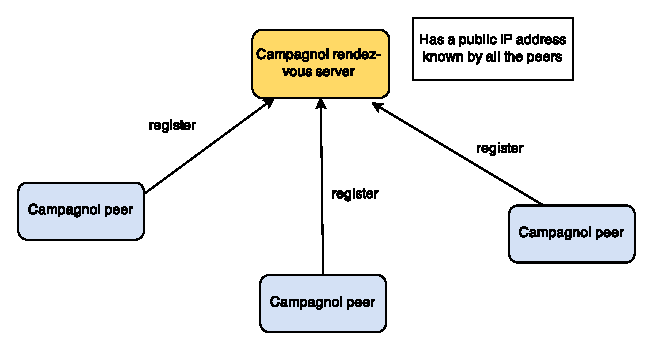
\includegraphics{images/campagnol-rdv.eps}
\caption{Every peer has to register with the rendez-vous}
\label{fig:campagnol-rdv}
\end{figure}

Whenever one of the peer wants to access another VPN IP, it contacts the rendez-vous server and asks for the real IP if it exists. Figure \ref{fig:campagnol-rdv2} presents these interactions. Once the IP address and the port of the corresponding peer have been retrieved, the DTLS handshake takes place.

\begin{figure}[!ht]
\centering
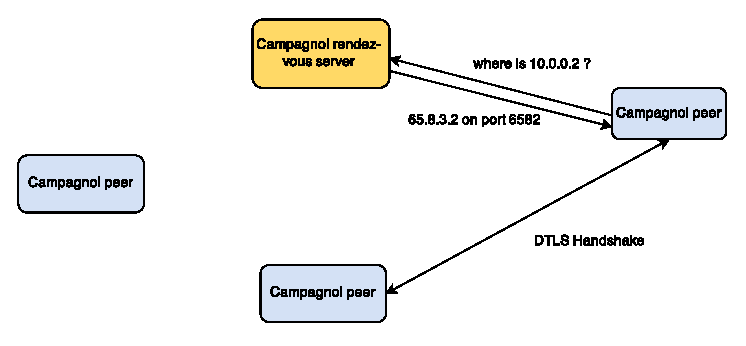
\includegraphics{images/campagnol-rdv2.eps}
\caption{Real IP acquisition through RDV server}
\label{fig:campagnol-rdv2}
\end{figure}

If we go deeper in the implementation, we notice that all the code is threaded and each thread has its own responsibility. For instance all the communications with the rendez-vous server and the other peers are using the same and only UDP socket. The thread handling the socket is then responsible to dispatch the packets to the other threads through a FIFO queue. Figure \ref{fig:campagnol-dtls} is depicting this behavior.

In order to know if a particular packet is DTLS, the record layer is extracted and the sender's IP address is matched against the list of known peers. It is then transmitted to the thread in charge of this session. The replies, if replies exist, are transmitted using again the same UDP socket.

\begin{figure}[!ht]
\centering
\includegraphics[width=\textwidth]{images/campagnol-overview.eps}
\caption{Campagnol DTLS communications}
\label{fig:campagnol-dtls}
\end{figure}


\section{wolfSSL integration difficulties}


We faced some difficulties trying to integrate successfully our modified library before we realized it was really difficult to both keep the decentralized aspect and bringing multipath. This would have required to redo the whole design of Campagnol and this was not our objective.

Here is a list of the main difficulties :

\begin{itemize}
\item The socket control : we modify wolfSSL and integrate the handling of the sockets when flows are  created or removed. It was a design choice but it brings some limitations on the existing application that could use this library. We need a full control of the sockets and the ability to create new ones that have the same status of the original one (used for the handshake). This is clearly not possible here because as shown in Figure \ref{fig:campagnol-dtls}, all the traffic is using the same non-connected UDP socket.
\item the CBIO compatibility : Campagnol originally uses OpenSSL \cite{openssl} with the CBIO. This is an I/O abstraction provided by OpenSSL which can be useful but is only partially supported by wolfSSL. The whole system of FIFO queues between threads is using this CBIO abstraction and we had to rethink about a system that could be compatible with wolfSSL.
\item The nature of sockets : Campagnol uses non-blocking, non-connected sockets. While our implementation is compatible with non-blocking sockets as we tried not to brake this feature inside the library, we absolutely need connected sockets (as wolfssl do) to work correctly. When we choose a flow to send a particular packet, we only give the socket number to the \texttt{sendto} method. Even if we could proceed differently, we have chosen this way because wolfSSL requires this in the first place.
\end{itemize}

For all these reasons, we decided to develop our own VPN application between a client and a server like OpenVPN. Campagnol was still useful because we had to understand how it works quite deeply and we were able to take some parts of the code for our application; namely, the TUN initialization and the bridge between the TUN and the SSL library.




